% !TEX encoding = UTF-8
% !TEX program = pdflatex
% !TEX root = InformationRetrieval.tex
% !TEX spellcheck = it-IT

% 6 Ottobre 2016

%\chapter{Rappresentazione dei documenti}
%\section{Analisi automatica del testo}

Tutto è iniziato quando George K. \textbf{Zipf}, uno studioso americano di linguistica ha formulato delle leggi empiriche che mettono in relazione la \textbf{frequenza di una parola} con la sua \textbf{forma} e \textbf{significato}. 
Solo in un secondo momento queste leggi sono state applicate all'indicizzazione dei documenti.

L'osservazione di partenza è stata quella che ci sono poche parole che sono veramente molto frequenti, come gli articoli, e che sono poco significative rispetto il contenuto informativo del documento. Ci sono poi tante parole poco frequenti, alcune delle quali sono fortemente correlate al contenuto informativo del documento. Il gioco è quindi quello di sfruttare al meglio tali parole.

Questo andamento può essere rappresentato graficamente, prima andando a contare le frequenze delle singole parole, per poi andare ad ordinarle da quella più frequente a quella meno frequente. La distribuzione così ottenuta è intera, ma può essere approssimata da un'iperbole.

Tipicamente in inglese:
\begin{itemize}
	\item Le due parole più frequenti sono \textit{the} e \textit{of}, mediamente sono il 10\% delle parole del documento.
	\item Le 6 parole più frequenti corrispondo a circa il 20\% delle occorrente e le 50 parole più frequenti corrispondo a circa il 40\% dei testi. Questo deriva dal fatto che la lingua deve essere ridondante in modo che sia facile da capire.
	\item Considerando un'insieme di documenti molto ampio, circa la metà delle singole parole di quel campione compare una sola volta. Queste sono parole più significative dal punto di vista dell'informazione. Tuttavia è necessario tenere conto che in questo insieme di parole possono comparire anche gli errori di battitura.
\end{itemize}

\subsection{Legge di Zipf}

La legge di Zipf afferma che dato un campione di testi e calcolata la frequenza $f$ delle parole, una volta che si sono messe le parole in ordine decrescente di frequenza, cioè si sono ordinate le parole in base al ragno \textit{r}, la distribuzione che si ottiene ha un andamento assimilabile ad una iperbole e si ha che

$$
r \times f = k
$$

ovvero la distribuzione è data da $ f = \cfrac{k}{r}$.

Se anziché ragionare in termini di frequenza assoluta si passa a considerare quella relativa, ovvero la probabilità osservata di occorrenza della parola, la legge di Zipf può essere riscritta come 

$$
r \times P_r = c
$$

Dove $P_r$ è la probabilità di occorrenza della parola che occupa il rango $r$-esimo e $c$ è una costante ($c = 0.1$ per l'inglese).

Si ha che per la lingua inglese $c \approx 0,1$ e l'iperbole che si ottiene è riportata in figura \ref{fig:zipf}

\begin{figure}[htbp]
\centering
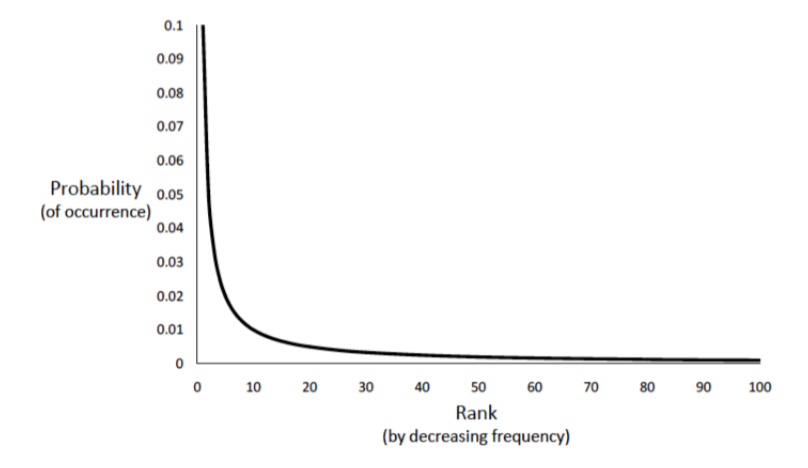
\includegraphics[width=0.55\linewidth]{images/l3-zipf}
\caption{Rango rispetto la probabilità di occorrenza assumendo valida la legge di Zipf con $c = 0.1$}\label{fig:zipf}
\end{figure}

\subsection{Indicazioni di H.P. Luhn}

L'idea per l'indicizzazione è quindi quella di definire due soglie di \textit{cut-off} per evitare di prendere in considerazione le parole troppo frequenti, perché poco significative, e quelle troppo poco, per limitare l'effetto degli errori di battitura.

Ogni parola ha un certo \textbf{resolving power}, ovvero una certa capacità di discriminare il contenuto del documento da quello degli altri e di caratterizzare il contenuto della collezione.

\begin{figure}[htbp]
	\centering
	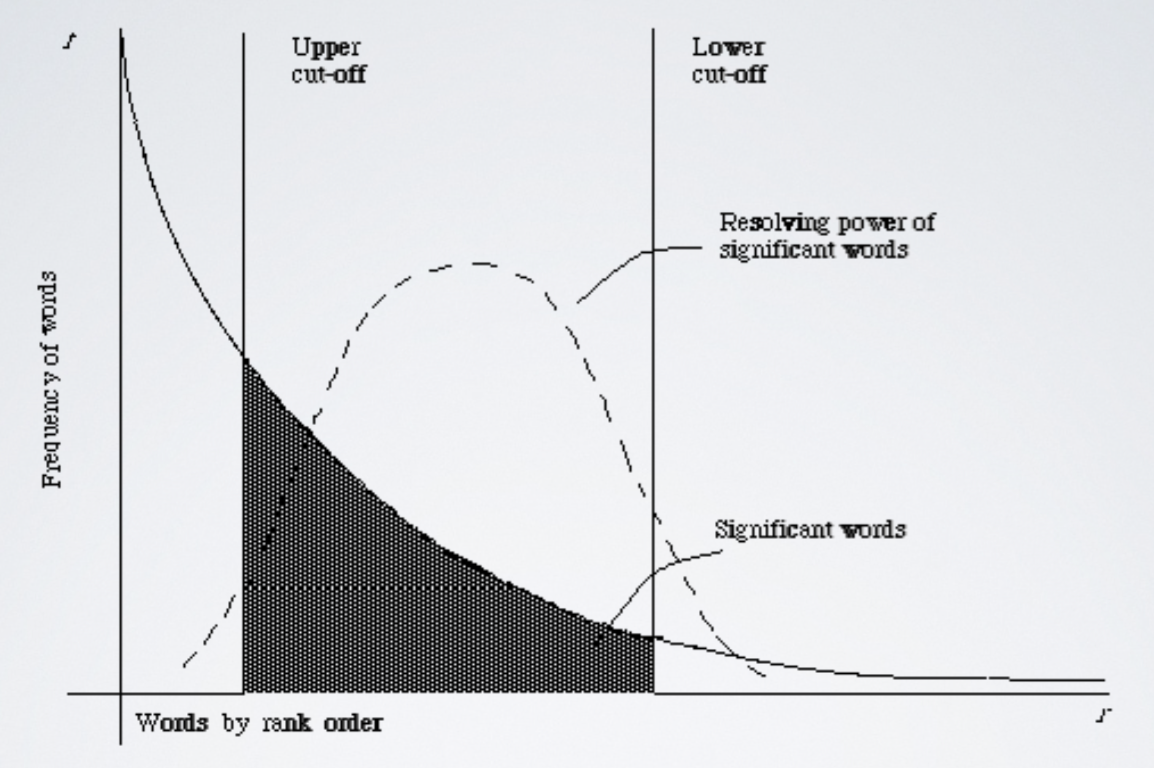
\includegraphics[width=0.55\linewidth]{images/l3-cutoff}
	\caption{Plot della curva $r \times f$ che evidenzia la posizione delle parole significative.}
\end{figure}

Questo vale per le collezioni generiche dei documenti, mentre se si parla di un argomento specifico si può dare maggiore peso a determinate parole. Ad esempio può capitare in che se viene preso in esame un manuale di MySQL è ovvio che le parole ``MySQL'' e  ``table'' compariranno tante volte anche se non sono articoli.

C'è anche un altro discorso relativo alla forma plurale, che in conteggio di frequenza vengono considerate come diverse, quando in realtà può essere che abbia lo stesso valore informativo della forma singolare. In alcuni casi è quindi opportuno sommare le occorrenze della forma plurale e di quella singolare.

Si ha quindi che i passi per applicare le indicazioni di Luhn sono:

\begin{itemize}
	\item Si calcoli la frequenza di ogni descrittore in ogni documento della collezione di riferimento. C'è inoltre da scegliere come trattare le parti di contorno dei documenti come l'indice, la premessa, ecc. tali parti tipicamente non vengono considerate.
	\item Si calcoli la frequenza totale di ogni descrittore.
	\item Si ordino i descrittori per frequenza decrescente.
	\item Si scelga una soglia di \textit{upper cut-off} e si rimuovano dalla lista i descrittori con frequenza superiore alla soglia. In questo modo si rimuovono gli articoli, le preposizioni, ecc.
	\item Si scelga un'altra soglia di \textit{lower cut-off} e si rimuovano dalla lista i descrittori con frequenza inferiore al valore di soglia. In questo modo si rimuovono i descrittori ``rumore''  o che non apportano alcun contribuito alla descrizione del contenuto.
\end{itemize}

\noindent Entrambe le soglie possono essere calcolate in modo euristico.

Le parole che vengo eliminate dalle soglie di cut-off vengono nominate \textbf{stop word} e sono raccolte nella lista che prende il nome di \textbf{stop list}.


\textbf{{\color{Red} Possibile esercizio:}} Domande relative alle osservazioni proposte da Zipf e Luhn.

\section{Indicizzazione}

L'indicizzazione ha l'obiettivo di rappresentare il contenuto informativo di un documento e nel tempo questo processo ha preso una struttura a fasi.

Il documento viene rappresentato da dei descrittori che vengono utilizzati per la costruzione degli indici, utili al reperimento dell'informazione.

Quindi l'indicizzazione fornisce automaticamente una rappresentazione più compatta e direttamente utilizzabile del contenuto informativo del documento. Gli indici sono utilizzati come surrogati del contenuto del documento durante la fase di reperimento.

L'indicizzazione può essere svolta:
\begin{itemize}
	\item manualmente
	\item in modo automatico
	\item in modo semi-automatico, quando è necessario intervenire all'interno del processo per prendere delle decisioni che non possono essere prese in modo automatico.
\end{itemize}

\noindent Tutti questi metodi funzionano estraendo direttamente dal documento le informazioni. Tuttavia possono essere estesi in modo che vengano presi in considerazione anche dei dizionari o delle meta-informazioni.

\begin{figure}[htbp]
	\centering
	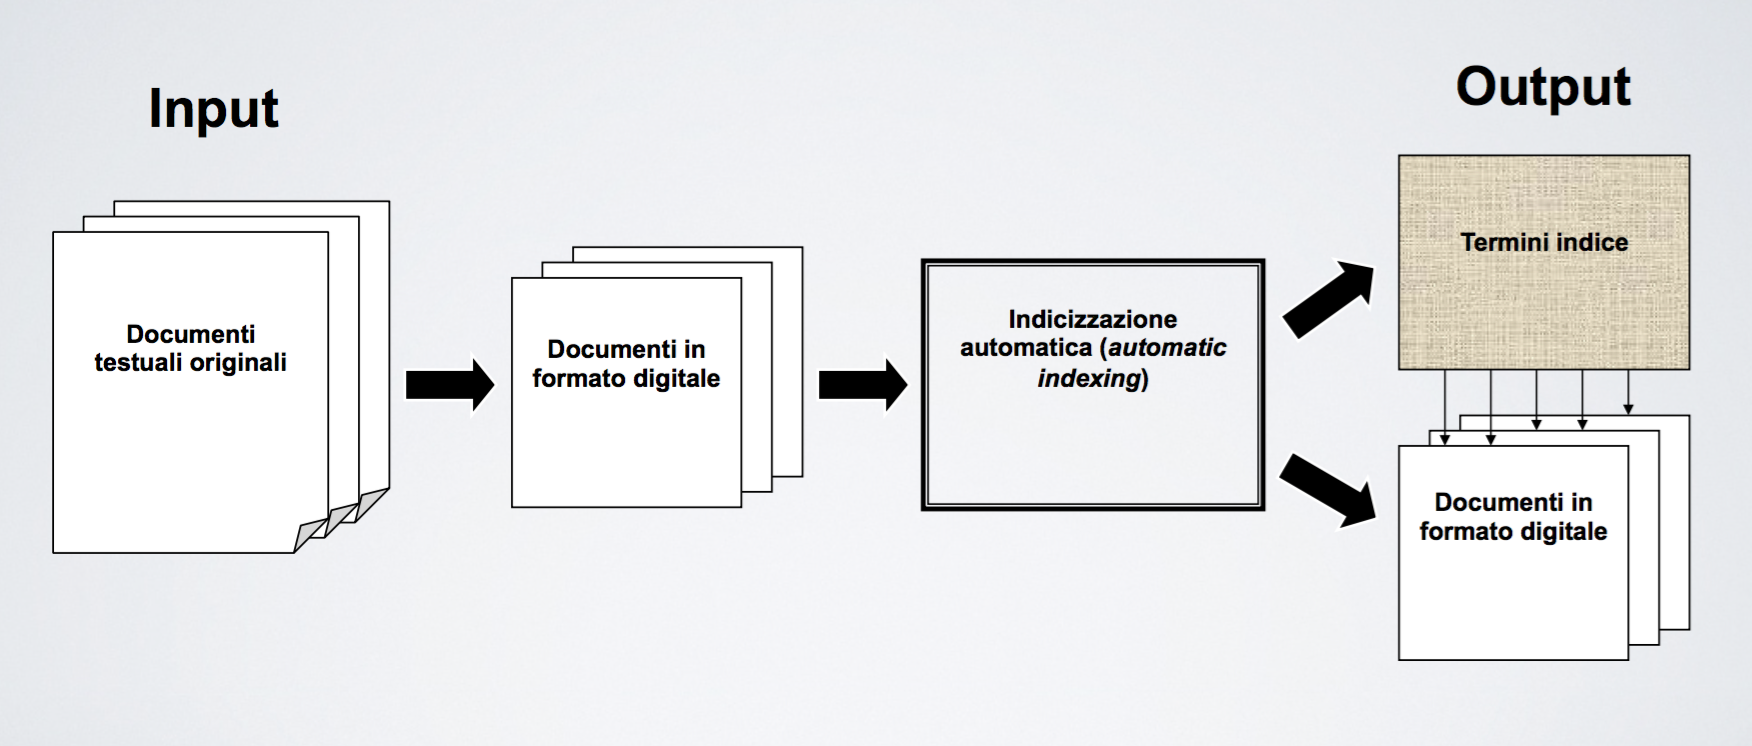
\includegraphics[width=0.7\linewidth]{images/l3-indicizzazione}
	\caption{Schema generale dell'indicizzazione}
\end{figure}

\subsection{Indicizzazione automatica dei testi}

L'indicizzazione automatica di un documento testuale è un processo che esamina automaticamente gli oggetti informativi (parole, frasi, didascalie, figure, ecc.) che compongono il documento e produce una lista di termini indice presenti nell'intera collezione dei documenti.

L'estrazione dei termini indice viene fatta da appositi algoritmi e, una volta estratti, questi vengono collegati ai diversi documenti che li contengono.
Così facendo durante il reperimento sarà sufficiente fare riferimento ai termini indice e non all'intera collezione.

\subsection{Attuazione dell'indicizzazione automatica}

L'indicizzazione automatica dei documenti testuali viene eseguita in più fasi, che devono essere attuate in sequenza:

\begin{enumerate}
	\item Analisi lessicale e selezione delle parole.
	\item Eventuale rimozione delle stop word.
	\item Riduzione delle parole originali alle rispettive radici (\textit{STEM}). Ad esempio le forme plurali vengono ridotte a quelle singolari.
	\item Composizione dei termini. Come ad esempio ``information retrieval''. Ovvero le parole vengono combinate tra loro quando si trovano ad una determinata distanza.
	\item Creazione dell'indice.
	\item Eventuale pesatura degli elementi dell'indice. 
\end{enumerate}

Alla fine di queste fasi l'indice sarà composto da parole, termini e frasi che noi riteniamo significative, assieme alle informazioni del peso che gli diamo e alla loro frequenza all'interno dei documenti.








